% Fig. 4.16 -- 二元常態聯合 pdf 由正上方俯瞰的灰階填色，兩面板。
% 書稿來源: mathstatch4.tex 第 5331 至 5380 行 (左面板) 與第 5383 至 5432 行
%   (右面板)。書稿把兩個 tikzpicture 各放進一個 .49\textwidth 的 minipage
%   橫排成一列 (第 5329 至 5434 行)，網頁併為一張兩面板圖。
%
% 這一張畫的就是 Fig. 4.15 那兩個曲面由正上方看下去的樣子: 函數、參數、
%   繪圖範圍、取樣點數與色階全部與 Fig. 4.15 的對應面板相同，只把視角改為
%   view={0}{90}。書稿雖然規劃時稱作等高線圖，實際畫的是 surf 俯瞰所形成的
%   灰階填色，圖上並沒有等高線，本檔照書稿保留灰階填色的作法 (候選稿的
%   fig-pending 註解已把改畫等高線列為待作者裁定，預設照書稿)。
%
% 繪圖函數同樣照書稿原樣保留，未改為真正的機率密度函數，理由與待裁定事項
%   見 bivariate-normal-surface.tex 的檔頭。俯瞰圖只看形狀不看高度，這一點
%   對本圖的外觀沒有影響。
%
% 書稿以 % 註解掉而未畫的部分一律不畫，項目與 Fig. 4.15 相同。
%
% 對書稿的三處調整:
%   1. colormap 由 whitegray 改為同色相的墨色濃淡 journalgray (CH3 規格 3.2)。
%   2. samples 由 50 改為 40 (CH3 規格 3.2 所定的產製規格)。
%   3. 兩軸標示的字級由書稿的 \LARGE 收為 \large，並把 x 軸標示下移 1.6mm、
%      y 軸標示左移 1.4mm，使標示與填色方塊的最短墨跡距離在 CH2 規格
%      第 1.3 節所定的 0.25cm 之上。書稿排成兩行的 x 軸標示照抄，
%      上行 $x$、下行 $(\rho = 0)$ 或 $(\rho = -0.8)$; y 軸標示照書稿旋轉 -90 度。
%      書稿另設而俯瞰時看不到的 z 軸標示不寫。
%
% 量測 (200 dpi 出圖逐像素量): 標示與填色方塊的最短距離 0.279cm，
%   在 0.25cm 之上。viewBox 寬 337.25，350px 之下放大 1.0378 倍、
%   620px 之下放大 1.8384 倍; 全圖沒有下標，最小可見字即 12pt 的軸名，
%   350px 之下合 12.4px、620px 之下合 22.0px，在 11px 門檻之上。
%
% 產製 (CH3 規格 3.2 的三維曲面路徑，-O 不可省):
%   latex -interaction=nonstopmode '\def\pgfsysdriver{pgfsys-dvisvgm.def}% Fig. 4.16 -- 二元常態聯合 pdf 由正上方俯瞰的灰階填色，兩面板。
% 書稿來源: mathstatch4.tex 第 5331 至 5380 行 (左面板) 與第 5383 至 5432 行
%   (右面板)。書稿把兩個 tikzpicture 各放進一個 .49\textwidth 的 minipage
%   橫排成一列 (第 5329 至 5434 行)，網頁併為一張兩面板圖。
%
% 這一張畫的就是 Fig. 4.15 那兩個曲面由正上方看下去的樣子: 函數、參數、
%   繪圖範圍、取樣點數與色階全部與 Fig. 4.15 的對應面板相同，只把視角改為
%   view={0}{90}。書稿雖然規劃時稱作等高線圖，實際畫的是 surf 俯瞰所形成的
%   灰階填色，圖上並沒有等高線，本檔照書稿保留灰階填色的作法 (候選稿的
%   fig-pending 註解已把改畫等高線列為待作者裁定，預設照書稿)。
%
% 繪圖函數同樣照書稿原樣保留，未改為真正的機率密度函數，理由與待裁定事項
%   見 bivariate-normal-surface.tex 的檔頭。俯瞰圖只看形狀不看高度，這一點
%   對本圖的外觀沒有影響。
%
% 書稿以 % 註解掉而未畫的部分一律不畫，項目與 Fig. 4.15 相同。
%
% 對書稿的三處調整:
%   1. colormap 由 whitegray 改為同色相的墨色濃淡 journalgray (CH3 規格 3.2)。
%   2. samples 由 50 改為 40 (CH3 規格 3.2 所定的產製規格)。
%   3. 兩軸標示的字級由書稿的 \LARGE 收為 \large，並把 x 軸標示下移 1.6mm、
%      y 軸標示左移 1.4mm，使標示與填色方塊的最短墨跡距離在 CH2 規格
%      第 1.3 節所定的 0.25cm 之上。書稿排成兩行的 x 軸標示照抄，
%      上行 $x$、下行 $(\rho = 0)$ 或 $(\rho = -0.8)$; y 軸標示照書稿旋轉 -90 度。
%      書稿另設而俯瞰時看不到的 z 軸標示不寫。
%
% 量測 (200 dpi 出圖逐像素量): 標示與填色方塊的最短距離 0.279cm，
%   在 0.25cm 之上。viewBox 寬 337.25，350px 之下放大 1.0378 倍、
%   620px 之下放大 1.8384 倍; 全圖沒有下標，最小可見字即 12pt 的軸名，
%   350px 之下合 12.4px、620px 之下合 22.0px，在 11px 門檻之上。
%
% 產製 (CH3 規格 3.2 的三維曲面路徑，-O 不可省):
%   latex -interaction=nonstopmode '\def\pgfsysdriver{pgfsys-dvisvgm.def}% Fig. 4.16 -- 二元常態聯合 pdf 由正上方俯瞰的灰階填色，兩面板。
% 書稿來源: mathstatch4.tex 第 5331 至 5380 行 (左面板) 與第 5383 至 5432 行
%   (右面板)。書稿把兩個 tikzpicture 各放進一個 .49\textwidth 的 minipage
%   橫排成一列 (第 5329 至 5434 行)，網頁併為一張兩面板圖。
%
% 這一張畫的就是 Fig. 4.15 那兩個曲面由正上方看下去的樣子: 函數、參數、
%   繪圖範圍、取樣點數與色階全部與 Fig. 4.15 的對應面板相同，只把視角改為
%   view={0}{90}。書稿雖然規劃時稱作等高線圖，實際畫的是 surf 俯瞰所形成的
%   灰階填色，圖上並沒有等高線，本檔照書稿保留灰階填色的作法 (候選稿的
%   fig-pending 註解已把改畫等高線列為待作者裁定，預設照書稿)。
%
% 繪圖函數同樣照書稿原樣保留，未改為真正的機率密度函數，理由與待裁定事項
%   見 bivariate-normal-surface.tex 的檔頭。俯瞰圖只看形狀不看高度，這一點
%   對本圖的外觀沒有影響。
%
% 書稿以 % 註解掉而未畫的部分一律不畫，項目與 Fig. 4.15 相同。
%
% 對書稿的三處調整:
%   1. colormap 由 whitegray 改為同色相的墨色濃淡 journalgray (CH3 規格 3.2)。
%   2. samples 由 50 改為 40 (CH3 規格 3.2 所定的產製規格)。
%   3. 兩軸標示的字級由書稿的 \LARGE 收為 \large，並把 x 軸標示下移 1.6mm、
%      y 軸標示左移 1.4mm，使標示與填色方塊的最短墨跡距離在 CH2 規格
%      第 1.3 節所定的 0.25cm 之上。書稿排成兩行的 x 軸標示照抄，
%      上行 $x$、下行 $(\rho = 0)$ 或 $(\rho = -0.8)$; y 軸標示照書稿旋轉 -90 度。
%      書稿另設而俯瞰時看不到的 z 軸標示不寫。
%
% 量測 (200 dpi 出圖逐像素量): 標示與填色方塊的最短距離 0.279cm，
%   在 0.25cm 之上。viewBox 寬 337.25，350px 之下放大 1.0378 倍、
%   620px 之下放大 1.8384 倍; 全圖沒有下標，最小可見字即 12pt 的軸名，
%   350px 之下合 12.4px、620px 之下合 22.0px，在 11px 門檻之上。
%
% 產製 (CH3 規格 3.2 的三維曲面路徑，-O 不可省):
%   latex -interaction=nonstopmode '\def\pgfsysdriver{pgfsys-dvisvgm.def}% Fig. 4.16 -- 二元常態聯合 pdf 由正上方俯瞰的灰階填色，兩面板。
% 書稿來源: mathstatch4.tex 第 5331 至 5380 行 (左面板) 與第 5383 至 5432 行
%   (右面板)。書稿把兩個 tikzpicture 各放進一個 .49\textwidth 的 minipage
%   橫排成一列 (第 5329 至 5434 行)，網頁併為一張兩面板圖。
%
% 這一張畫的就是 Fig. 4.15 那兩個曲面由正上方看下去的樣子: 函數、參數、
%   繪圖範圍、取樣點數與色階全部與 Fig. 4.15 的對應面板相同，只把視角改為
%   view={0}{90}。書稿雖然規劃時稱作等高線圖，實際畫的是 surf 俯瞰所形成的
%   灰階填色，圖上並沒有等高線，本檔照書稿保留灰階填色的作法 (候選稿的
%   fig-pending 註解已把改畫等高線列為待作者裁定，預設照書稿)。
%
% 繪圖函數同樣照書稿原樣保留，未改為真正的機率密度函數，理由與待裁定事項
%   見 bivariate-normal-surface.tex 的檔頭。俯瞰圖只看形狀不看高度，這一點
%   對本圖的外觀沒有影響。
%
% 書稿以 % 註解掉而未畫的部分一律不畫，項目與 Fig. 4.15 相同。
%
% 對書稿的三處調整:
%   1. colormap 由 whitegray 改為同色相的墨色濃淡 journalgray (CH3 規格 3.2)。
%   2. samples 由 50 改為 40 (CH3 規格 3.2 所定的產製規格)。
%   3. 兩軸標示的字級由書稿的 \LARGE 收為 \large，並把 x 軸標示下移 1.6mm、
%      y 軸標示左移 1.4mm，使標示與填色方塊的最短墨跡距離在 CH2 規格
%      第 1.3 節所定的 0.25cm 之上。書稿排成兩行的 x 軸標示照抄，
%      上行 $x$、下行 $(\rho = 0)$ 或 $(\rho = -0.8)$; y 軸標示照書稿旋轉 -90 度。
%      書稿另設而俯瞰時看不到的 z 軸標示不寫。
%
% 量測 (200 dpi 出圖逐像素量): 標示與填色方塊的最短距離 0.279cm，
%   在 0.25cm 之上。viewBox 寬 337.25，350px 之下放大 1.0378 倍、
%   620px 之下放大 1.8384 倍; 全圖沒有下標，最小可見字即 12pt 的軸名，
%   350px 之下合 12.4px、620px 之下合 22.0px，在 11px 門檻之上。
%
% 產製 (CH3 規格 3.2 的三維曲面路徑，-O 不可省):
%   latex -interaction=nonstopmode '\def\pgfsysdriver{pgfsys-dvisvgm.def}\input{bivariate-normal-contours.tex}'
%   dvisvgm -O -d2 -n -o ../../images/teaching-topics/bivariate-normal-contours.svg bivariate-normal-contours.dvi

\documentclass[tikz,border=2pt]{standalone}
\usepackage{amsmath}
\usepackage{amssymb}
\usepackage{xcolor}
\usepackage{pgfplots}
\usepgfplotslibrary{groupplots}
\pgfplotsset{compat=1.18}

\definecolor{journalink}{HTML}{1F1C18}
\definecolor{journalmuted}{HTML}{8A7F72}
\definecolor{journalaccent}{HTML}{9C2D2D}

\DeclareMathSizes{12}{12}{11}{10}

%% 書稿用 whitegray 灰階曲面; 本站改用同一色相的墨色濃淡，
%% 與其他圖的主線色 journalink 相稱。
\pgfplotsset{
  colormap={journalgray}{color(0cm)=(white); color(1cm)=(journalink)}
}

\pgfplotsset{
  toppanel/.style={
    axis line style={draw=none},
    colormap name=journalgray,
    scale only axis,
    width=5.0cm,
    height=5.0cm,
    view={0}{90},
    enlargelimits=false,
    domain=0:4,
    y domain=0:4,
    samples=40,
    ylabel={$y$},
    label style={journalink, font=\large},
    tick style={draw=none},
    xtick=\empty,
    ytick=\empty,
    ztick=\empty,
    ylabel style={rotate=-90, xshift=-1.4mm},
    xlabel style={yshift=-1.6mm},
  },
}

\begin{document}
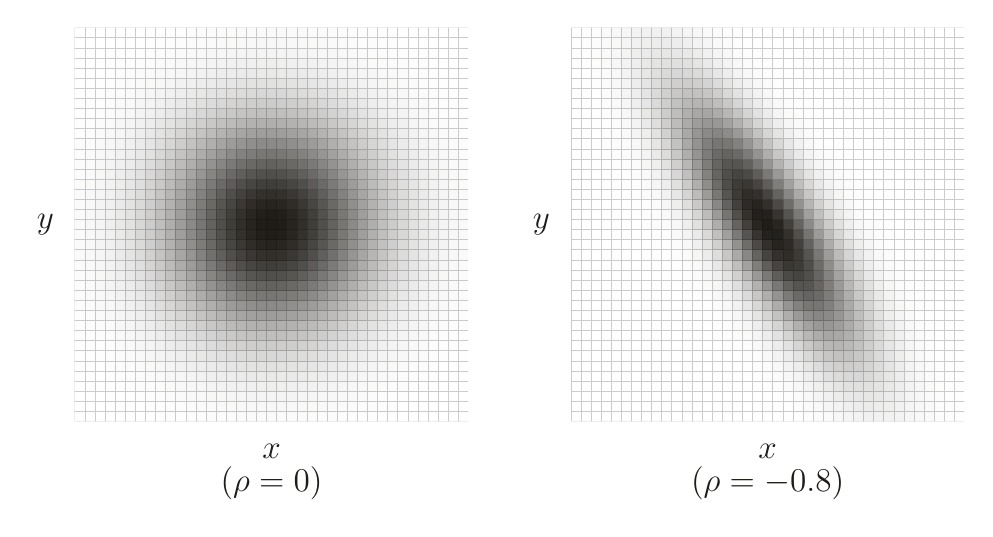
\begin{tikzpicture}[
    declare function={mu1=2;},
    declare function={mu2=2;},
    %% 零相關的那一個: 書稿第 5337 至 5338 行
    declare function={bivarA(\ma,\sa,\mb,\sb)=
        1/(2*pi*\sa*\sb) * exp(-((x-\ma)^2/\sa^2 + (y-\mb)^2/\sb^2))/2;},
    %% 負相關的那一個: 書稿第 5389 至 5390 行
    declare function={bivarB(\ma,\sa,\mb,\sb,\rr)=
        1/(2*pi*\sa*\sb*sqrt(1-\rr^2)) * exp(-((x-\ma)^2/\sa^2 + (y-\mb)^2/\sb^2 - 2*\rr*((x-\ma)/\sa)*((y-\mb)/\sb)))/2;}]
\begin{groupplot}[
  group style={group name=g, group size=2 by 1, horizontal sep=1.3cm},
  toppanel,
]

%% 左面板: 相關係數為零，俯瞰所見為一團正圓形
\nextgroupplot[xlabel={\shortstack{$x$ \\ $(\rho = 0)$}}]
\addplot3[surf, draw=journalink, line width=0.2pt] {bivarA(mu1,1,mu2,1)};

%% 右面板: 相關係數為負，俯瞰所見為一團由左上往右下傾斜的橢圓形
\nextgroupplot[xlabel={\shortstack{$x$ \\ $(\rho = -0.8)$}}]
\addplot3[surf, draw=journalink, line width=0.2pt] {bivarB(mu1,0.5,mu2,0.7,-0.8)};

\end{groupplot}
\end{tikzpicture}
\end{document}
'
%   dvisvgm -O -d2 -n -o ../../images/teaching-topics/bivariate-normal-contours.svg bivariate-normal-contours.dvi

\documentclass[tikz,border=2pt]{standalone}
\usepackage{amsmath}
\usepackage{amssymb}
\usepackage{xcolor}
\usepackage{pgfplots}
\usepgfplotslibrary{groupplots}
\pgfplotsset{compat=1.18}

\definecolor{journalink}{HTML}{1F1C18}
\definecolor{journalmuted}{HTML}{8A7F72}
\definecolor{journalaccent}{HTML}{9C2D2D}

\DeclareMathSizes{12}{12}{11}{10}

%% 書稿用 whitegray 灰階曲面; 本站改用同一色相的墨色濃淡，
%% 與其他圖的主線色 journalink 相稱。
\pgfplotsset{
  colormap={journalgray}{color(0cm)=(white); color(1cm)=(journalink)}
}

\pgfplotsset{
  toppanel/.style={
    axis line style={draw=none},
    colormap name=journalgray,
    scale only axis,
    width=5.0cm,
    height=5.0cm,
    view={0}{90},
    enlargelimits=false,
    domain=0:4,
    y domain=0:4,
    samples=40,
    ylabel={$y$},
    label style={journalink, font=\large},
    tick style={draw=none},
    xtick=\empty,
    ytick=\empty,
    ztick=\empty,
    ylabel style={rotate=-90, xshift=-1.4mm},
    xlabel style={yshift=-1.6mm},
  },
}

\begin{document}
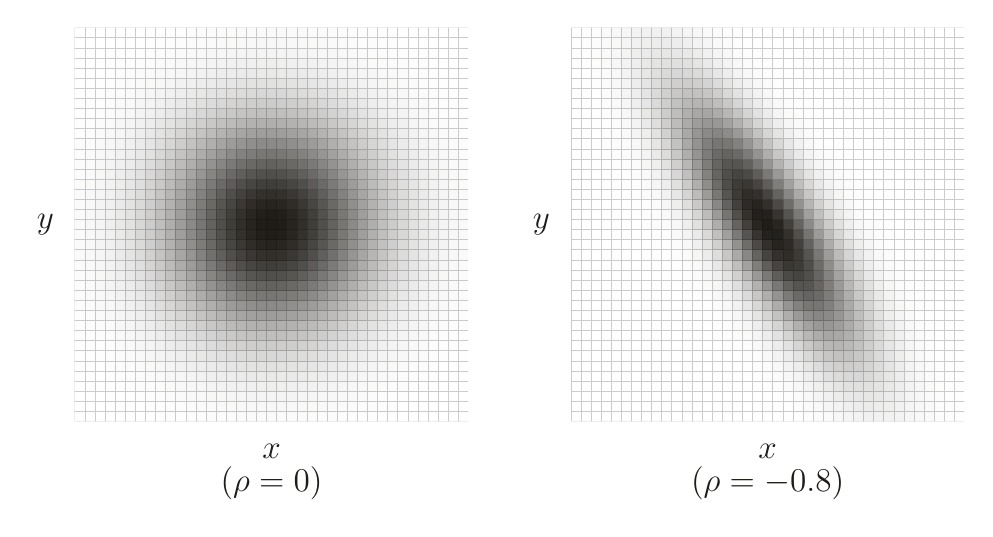
\begin{tikzpicture}[
    declare function={mu1=2;},
    declare function={mu2=2;},
    %% 零相關的那一個: 書稿第 5337 至 5338 行
    declare function={bivarA(\ma,\sa,\mb,\sb)=
        1/(2*pi*\sa*\sb) * exp(-((x-\ma)^2/\sa^2 + (y-\mb)^2/\sb^2))/2;},
    %% 負相關的那一個: 書稿第 5389 至 5390 行
    declare function={bivarB(\ma,\sa,\mb,\sb,\rr)=
        1/(2*pi*\sa*\sb*sqrt(1-\rr^2)) * exp(-((x-\ma)^2/\sa^2 + (y-\mb)^2/\sb^2 - 2*\rr*((x-\ma)/\sa)*((y-\mb)/\sb)))/2;}]
\begin{groupplot}[
  group style={group name=g, group size=2 by 1, horizontal sep=1.3cm},
  toppanel,
]

%% 左面板: 相關係數為零，俯瞰所見為一團正圓形
\nextgroupplot[xlabel={\shortstack{$x$ \\ $(\rho = 0)$}}]
\addplot3[surf, draw=journalink, line width=0.2pt] {bivarA(mu1,1,mu2,1)};

%% 右面板: 相關係數為負，俯瞰所見為一團由左上往右下傾斜的橢圓形
\nextgroupplot[xlabel={\shortstack{$x$ \\ $(\rho = -0.8)$}}]
\addplot3[surf, draw=journalink, line width=0.2pt] {bivarB(mu1,0.5,mu2,0.7,-0.8)};

\end{groupplot}
\end{tikzpicture}
\end{document}
'
%   dvisvgm -O -d2 -n -o ../../images/teaching-topics/bivariate-normal-contours.svg bivariate-normal-contours.dvi

\documentclass[tikz,border=2pt]{standalone}
\usepackage{amsmath}
\usepackage{amssymb}
\usepackage{xcolor}
\usepackage{pgfplots}
\usepgfplotslibrary{groupplots}
\pgfplotsset{compat=1.18}

\definecolor{journalink}{HTML}{1F1C18}
\definecolor{journalmuted}{HTML}{8A7F72}
\definecolor{journalaccent}{HTML}{9C2D2D}

\DeclareMathSizes{12}{12}{11}{10}

%% 書稿用 whitegray 灰階曲面; 本站改用同一色相的墨色濃淡，
%% 與其他圖的主線色 journalink 相稱。
\pgfplotsset{
  colormap={journalgray}{color(0cm)=(white); color(1cm)=(journalink)}
}

\pgfplotsset{
  toppanel/.style={
    axis line style={draw=none},
    colormap name=journalgray,
    scale only axis,
    width=5.0cm,
    height=5.0cm,
    view={0}{90},
    enlargelimits=false,
    domain=0:4,
    y domain=0:4,
    samples=40,
    ylabel={$y$},
    label style={journalink, font=\large},
    tick style={draw=none},
    xtick=\empty,
    ytick=\empty,
    ztick=\empty,
    ylabel style={rotate=-90, xshift=-1.4mm},
    xlabel style={yshift=-1.6mm},
  },
}

\begin{document}
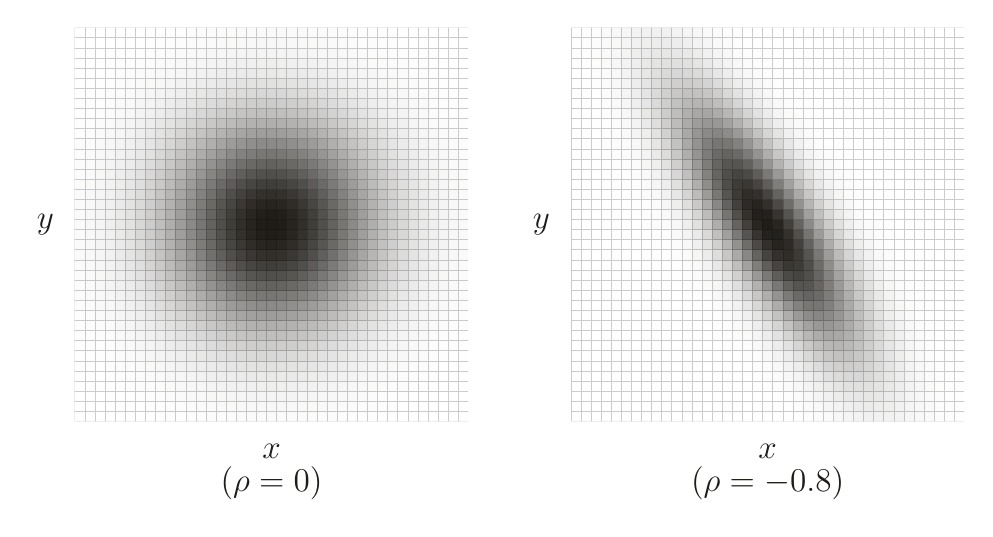
\begin{tikzpicture}[
    declare function={mu1=2;},
    declare function={mu2=2;},
    %% 零相關的那一個: 書稿第 5337 至 5338 行
    declare function={bivarA(\ma,\sa,\mb,\sb)=
        1/(2*pi*\sa*\sb) * exp(-((x-\ma)^2/\sa^2 + (y-\mb)^2/\sb^2))/2;},
    %% 負相關的那一個: 書稿第 5389 至 5390 行
    declare function={bivarB(\ma,\sa,\mb,\sb,\rr)=
        1/(2*pi*\sa*\sb*sqrt(1-\rr^2)) * exp(-((x-\ma)^2/\sa^2 + (y-\mb)^2/\sb^2 - 2*\rr*((x-\ma)/\sa)*((y-\mb)/\sb)))/2;}]
\begin{groupplot}[
  group style={group name=g, group size=2 by 1, horizontal sep=1.3cm},
  toppanel,
]

%% 左面板: 相關係數為零，俯瞰所見為一團正圓形
\nextgroupplot[xlabel={\shortstack{$x$ \\ $(\rho = 0)$}}]
\addplot3[surf, draw=journalink, line width=0.2pt] {bivarA(mu1,1,mu2,1)};

%% 右面板: 相關係數為負，俯瞰所見為一團由左上往右下傾斜的橢圓形
\nextgroupplot[xlabel={\shortstack{$x$ \\ $(\rho = -0.8)$}}]
\addplot3[surf, draw=journalink, line width=0.2pt] {bivarB(mu1,0.5,mu2,0.7,-0.8)};

\end{groupplot}
\end{tikzpicture}
\end{document}
'
%   dvisvgm -O -d2 -n -o ../../images/teaching-topics/bivariate-normal-contours.svg bivariate-normal-contours.dvi

\documentclass[tikz,border=2pt]{standalone}
\usepackage{amsmath}
\usepackage{amssymb}
\usepackage{xcolor}
\usepackage{pgfplots}
\usepgfplotslibrary{groupplots}
\pgfplotsset{compat=1.18}

\definecolor{journalink}{HTML}{1F1C18}
\definecolor{journalmuted}{HTML}{8A7F72}
\definecolor{journalaccent}{HTML}{9C2D2D}

\DeclareMathSizes{12}{12}{11}{10}

%% 書稿用 whitegray 灰階曲面; 本站改用同一色相的墨色濃淡，
%% 與其他圖的主線色 journalink 相稱。
\pgfplotsset{
  colormap={journalgray}{color(0cm)=(white); color(1cm)=(journalink)}
}

\pgfplotsset{
  toppanel/.style={
    axis line style={draw=none},
    colormap name=journalgray,
    scale only axis,
    width=5.0cm,
    height=5.0cm,
    view={0}{90},
    enlargelimits=false,
    domain=0:4,
    y domain=0:4,
    samples=40,
    ylabel={$y$},
    label style={journalink, font=\large},
    tick style={draw=none},
    xtick=\empty,
    ytick=\empty,
    ztick=\empty,
    ylabel style={rotate=-90, xshift=-1.4mm},
    xlabel style={yshift=-1.6mm},
  },
}

\begin{document}
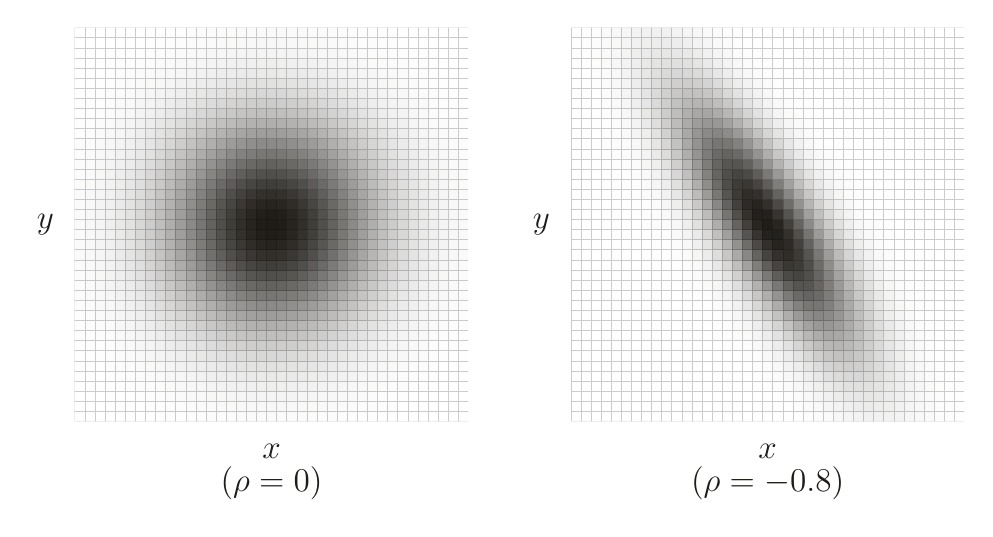
\begin{tikzpicture}[
    declare function={mu1=2;},
    declare function={mu2=2;},
    %% 零相關的那一個: 書稿第 5337 至 5338 行
    declare function={bivarA(\ma,\sa,\mb,\sb)=
        1/(2*pi*\sa*\sb) * exp(-((x-\ma)^2/\sa^2 + (y-\mb)^2/\sb^2))/2;},
    %% 負相關的那一個: 書稿第 5389 至 5390 行
    declare function={bivarB(\ma,\sa,\mb,\sb,\rr)=
        1/(2*pi*\sa*\sb*sqrt(1-\rr^2)) * exp(-((x-\ma)^2/\sa^2 + (y-\mb)^2/\sb^2 - 2*\rr*((x-\ma)/\sa)*((y-\mb)/\sb)))/2;}]
\begin{groupplot}[
  group style={group name=g, group size=2 by 1, horizontal sep=1.3cm},
  toppanel,
]

%% 左面板: 相關係數為零，俯瞰所見為一團正圓形
\nextgroupplot[xlabel={\shortstack{$x$ \\ $(\rho = 0)$}}]
\addplot3[surf, draw=journalink, line width=0.2pt] {bivarA(mu1,1,mu2,1)};

%% 右面板: 相關係數為負，俯瞰所見為一團由左上往右下傾斜的橢圓形
\nextgroupplot[xlabel={\shortstack{$x$ \\ $(\rho = -0.8)$}}]
\addplot3[surf, draw=journalink, line width=0.2pt] {bivarB(mu1,0.5,mu2,0.7,-0.8)};

\end{groupplot}
\end{tikzpicture}
\end{document}
